\documentclass[12pt]{article}
\usepackage{amsmath}
\usepackage{amsfonts}
\usepackage{parskip}
\usepackage{amsthm}
\usepackage{thmtools}
\usepackage[headheight=15pt]{geometry}
\geometry{a4paper, left=20mm, right=20mm, top=30mm, bottom=30mm}
\usepackage{graphicx}
\usepackage{bm} % for bold font in math mode - command is \bm{text}
\usepackage{enumitem}
\usepackage{fancyhdr}
\usepackage{amssymb} % for stacked arrows and other shit
\pagestyle{fancy}
\usepackage{changepage}
\usepackage{mathcomp}
\usepackage{tcolorbox}

\declaretheoremstyle[headfont=\normalfont]{normal}
\declaretheorem[style=normal]{Theorem}
\declaretheorem[style=normal]{Proposition}
\declaretheorem[style=normal]{Lemma}
\newcounter{ProofCounter}
\newcounter{ClaimCounter}[ProofCounter]
\newcounter{SubClaimCounter}[ClaimCounter]
\newenvironment{Proof}{\stepcounter{ProofCounter}\textsc{Proof.}}{\hfill$\square$}
\newenvironment{claim}[1]{\vspace{1mm}\stepcounter{ClaimCounter}\par\noindent\underline{\bf Claim \theClaimCounter:}\space#1}{}
\newenvironment{claimproof}[1]{\par\noindent\underline{Proof of claim \theClaimCounter:}\space#1}{\hfill $\blacksquare$ Claim \theClaimCounter}
\newenvironment{subclaim}[1]{\stepcounter{SubClaimCounter}\par\noindent\emph{Subclaim \theClaimCounter.\theSubClaimCounter:}\space#1}{}
% \newenvironment{subclaimproof}[1]{\begin{adjustwidth}{2em}{0pt}\par\noindent\emph{Proof of subclaim \theClaimCounter.\theSubClaimCounter:}\space#1}{\hfill
% $\blacksquare$ \emph{Subclaim \theClaimCounter.\theSubClaimCounter}\vspace{5mm}\end{adjustwidth}}
\newenvironment{subclaimproof}[1]{\par\noindent\emph{Proof of subclaim \theClaimCounter.\theSubClaimCounter:}\space#1}{\hfill
$\Diamond$ \emph{Subclaim \theClaimCounter.\theSubClaimCounter}}

\allowdisplaybreaks{}

% chktex-file 3

\title{STAT 520: Assignment 3}
\author{Evan P. Walsh}
\makeatletter
\makeatother
\lhead{Evan P. Walsh}
\chead{STAT 520: Assignment 3}
\rhead{\thepage}
\cfoot{}

\begin{document}
% \maketitle


\subsection*{Assignment 3.1}

\begin{enumerate}
  \item We define the random variables $Y_{1}, \dots, Y_{n}$ so that $Y_i$ is associated with the blood concentration of oxychlordane (OXY) in gull
    $i$ and the covariates $x_{1}, \dots, x_{n}$ such that $x_{i}$ is the body mass (in grams) of gull $i$. Then each $Y_{i}$ has support in the non-negative
    reals since concentration cannot be negative.

  \item In choosing a random model component we first need to make sure that the support of the model matches the support of the random variables we
    have defined. Thus a random model component with support in the non-negative reals is natural. This gives us several options, including Gamma and
    Inverse Gaussian. To determine which is the most appropriate, we 
    create a Box-Cox plot of the log of means 
    versus the log standard deviation of the response in 5 different bins, as shown below in Figure \ref{fig:1}.

    \begin{figure}[h]
      \caption{\emph{Box-Cot plot produced using the function \texttt{regmeanvar}.}}
      \centering
      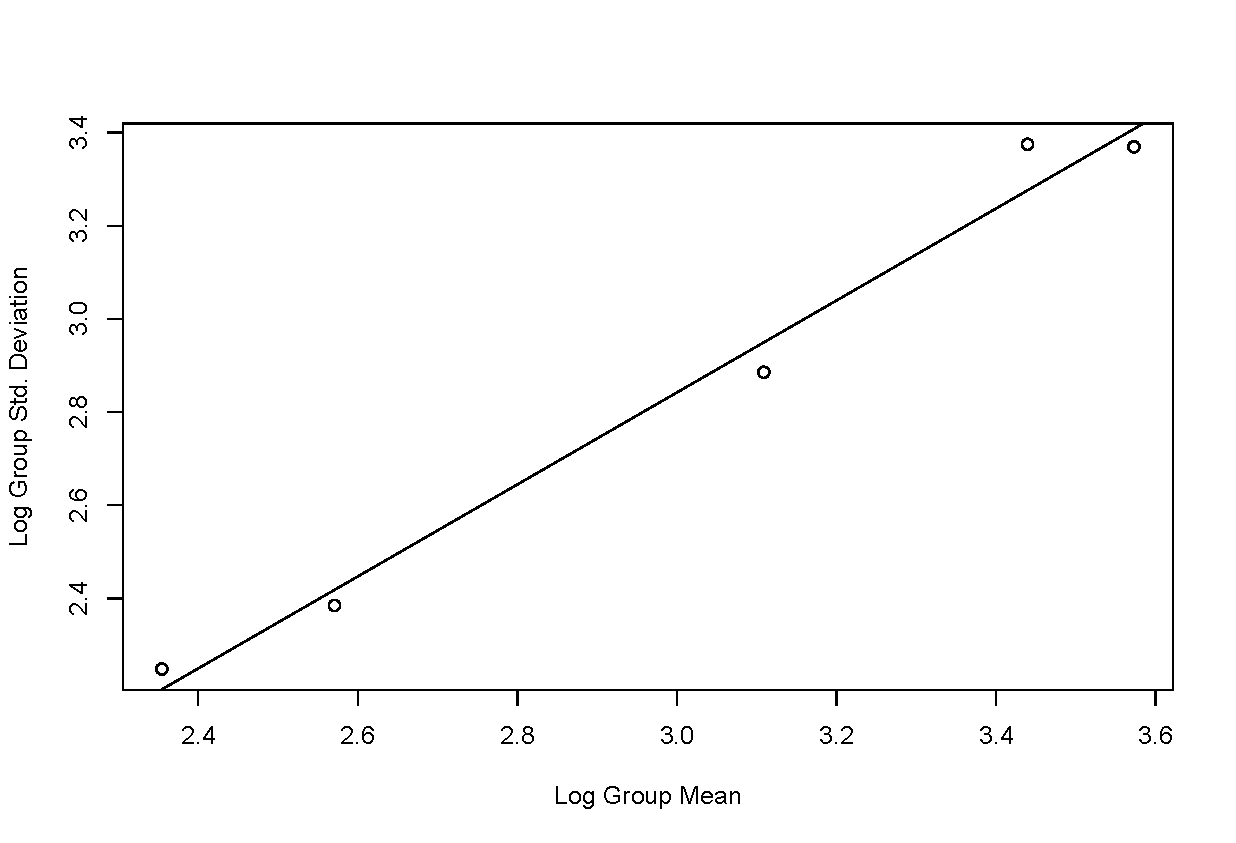
\includegraphics[width=.82\textwidth]{./figures/hw03_regmeanvar.pdf}
      \label{fig:1}
    \end{figure}

    The slope of the best fit line in Figure 1 is 0.988, suggesting that a Gamma random component is appropriate.

  \item To determine the appropriate link function, we plot various tranformations of the response variable OXY against the covariate, body mass.
    Figure \ref{fig:2} shows a log transformation of the response which results in a reasonably linear trend in the data. Thus we decide to use the
    log link.
    
    \begin{figure}[h]
      \caption{\emph{Log transformed data.}}
      \centering
      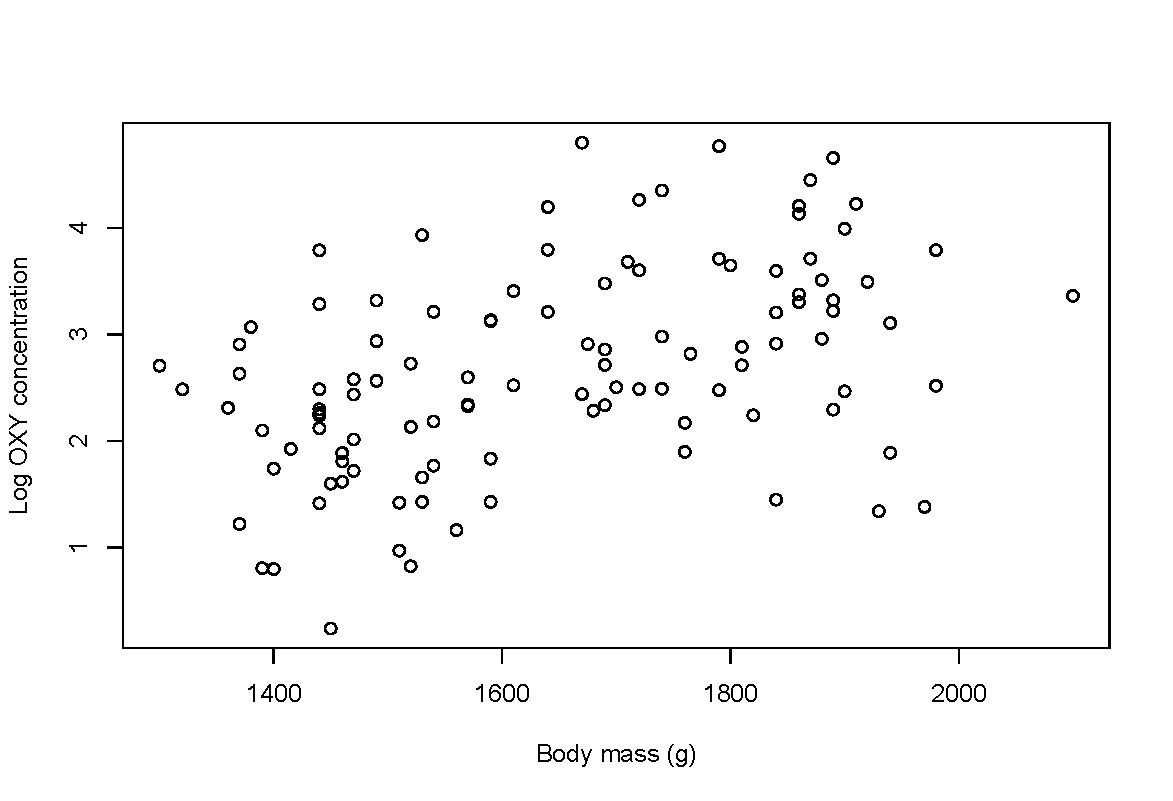
\includegraphics[width=.82\textwidth]{./figures/hw03_log_link.pdf}
      \label{fig:2}
    \end{figure}


  \item We fit a glm using the R function \texttt{basicglm} with a Gamma random component and a log link function. The results are summarized below in
    the Table 1, which includes 95\% Wald Theory intervals for the parameters $\beta_0$ and $\beta_1$. We also report the unscaled deviance $D_{u}$
    and the scaled deviance $D_{s}$.
    A scatterplot of the data along with the estimated expectation function is shown in Figure \ref{fig:3}.

    \begin{table}[h!]
      \caption{\emph{Results of glm fit to OXY with body mass as a covariate. Here $D_{u}$ represents the unscaled deviance while $D_{s}$ represents the
      scaled deviance.}}
      \vspace{.5cm}
      \centering
      \begin{tabular}{c|c|c|c|c|c|c|c}
        \hline
        $\hat{\phi}$ & $\hat{\beta_0}$ & $\hat{\beta_{1}}$ & 95\% CI for $\hat{\beta_0}$ & 95\% CI for $\hat{\beta_1}$ & $D_{u}$ & $D_{s}$ &
        $\ell(\hat{\beta_0}, \hat{\beta_1}, \hat{\phi})$ \\
        \hline
        $1.1673$ & $-0.9606$ & $0.0024$ & $(-2.4765, 0.5553)$ & $(0.0015, 0.0033)$ & 76.5991 & 89.4139 & $-144.0595$ \\
        \hline
      \end{tabular}
      \label{tab:1}
    \end{table}


    \begin{figure}[h!]
      \caption{\emph{Scatterplot of data with fitted expectation function.}}
      \centering
      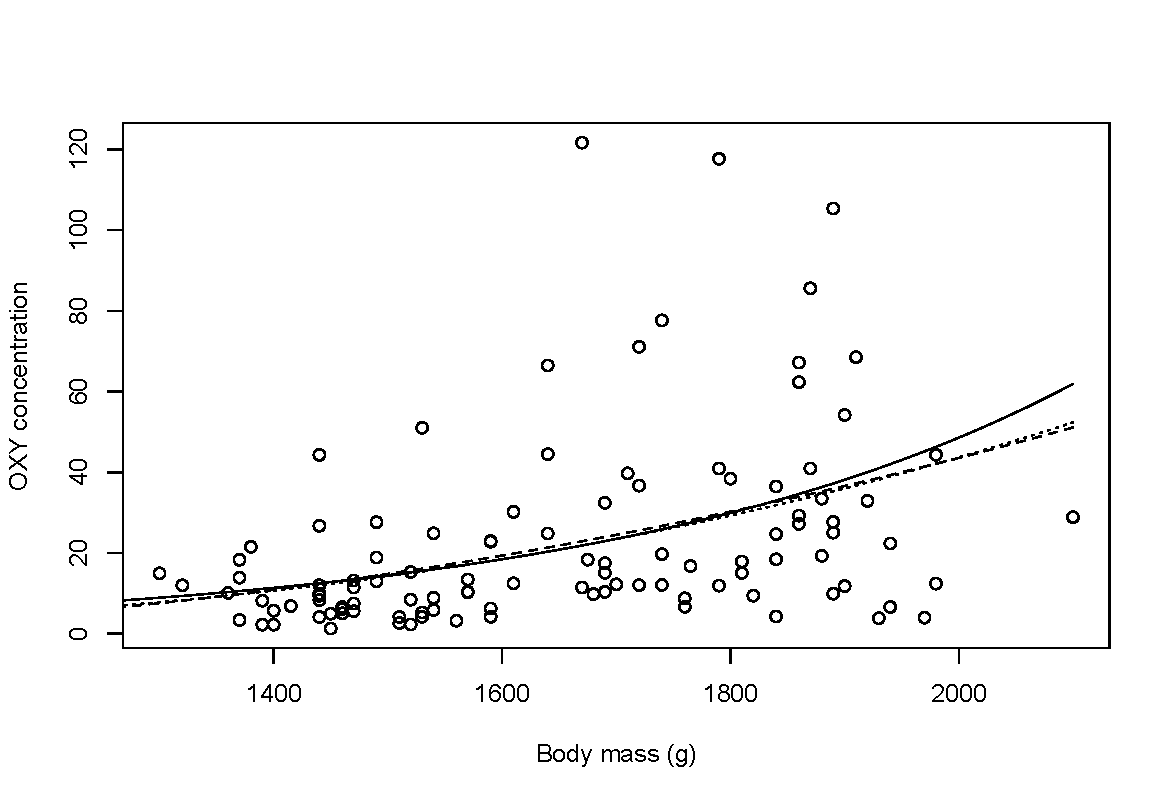
\includegraphics[width=.8\textwidth]{./figures/hw03_fitted.pdf}
      \label{fig:3}
    \end{figure}
\end{enumerate}


\newpage


\subsection*{Assignment 3.2}

\begin{enumerate}
  \item For this part of the assignment we simulated data coming from a generalized linear model with a binary random component and a complementary
    log-log link function. We used the regression coefficients $\beta_0 = -5$ and $\beta_1 = 0.14$. The results of fitting the same model to the
    simulated data as from which they were generated are displayed in Table 2. Note that we only report one deviance statistic and omit the estimated
    $\phi$ since $\phi = 1$, which implies that the unscaled deviance $D_{u}$ is equal to the scaled deviance $D_{s}$. A scatterplot with the estimated expectation function is also shown in Figure 4.

    \begin{table}[h]
      \caption{\emph{Results of glm fit to OXY with body mass as a covariate. Here $D$ represents both the unscaled and scaled deviance.}}
      \vspace{.5cm}
      \centering
      \begin{tabular}{c|c|c|c|c|c}
        \hline
        $\hat{\beta_0}$ & $\hat{\beta_{1}}$ & 95\% CI for $\hat{\beta_0}$ & 95\% CI for $\hat{\beta_1}$ & $D$ & 
        $\ell(\hat{\beta_0}, \hat{\beta_1}, \hat{\phi})$ \\
        \hline
        $-4.9082$ & $0.1442$ & $(-7.3544,-2.4620)$ & $(0.0727, 0.2157)$ & 31.920 & $-15.9601$ \\
        \hline
      \end{tabular}
      \label{tab:2}
    \end{table}

    \begin{figure}[h]
      \caption{\emph{Scatterplot of the simulated data with the estimated expectation function.}}

      \centering
      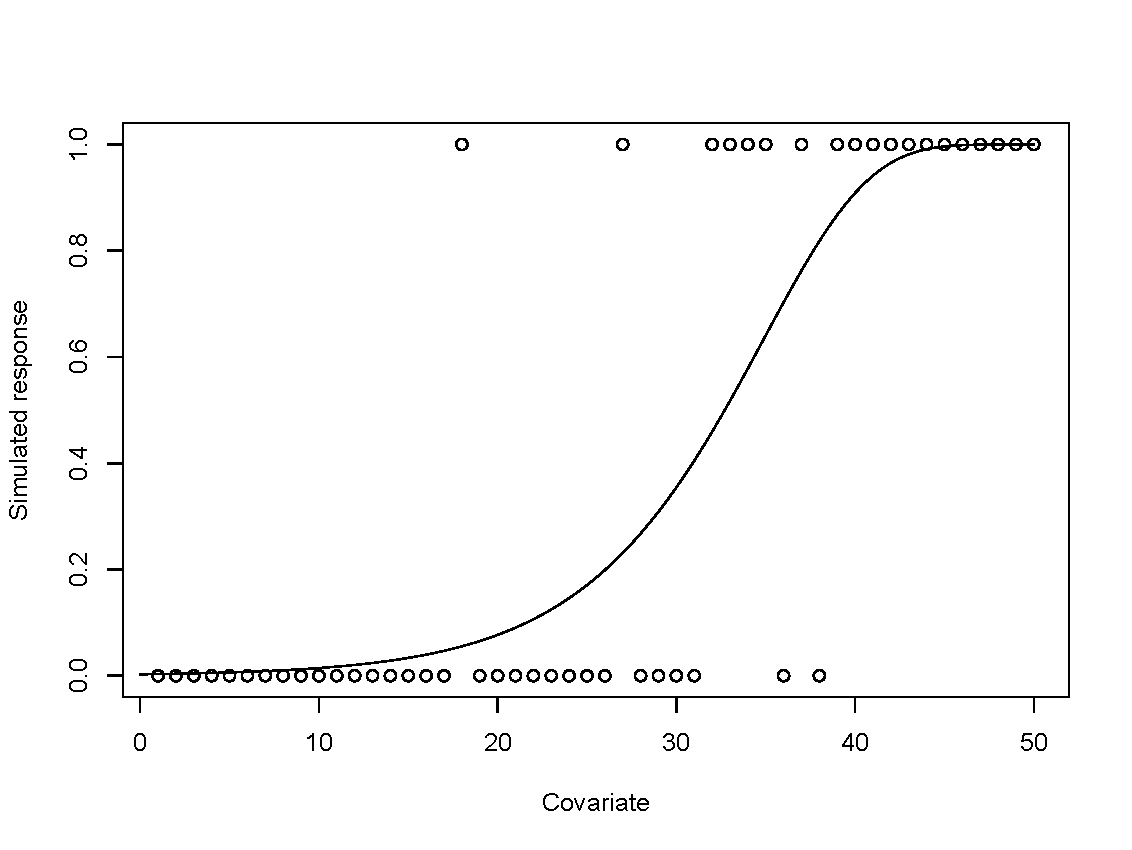
\includegraphics[width=.8\textwidth]{./figures/hw03_2_fitted.pdf}
      \label{fig:4}
    \end{figure}

  \item  Lastly we compute 95\% pointwise confidence bands for the expectation function. We do this using the multivariate delta method on the
    inverse of the link function. The results are displayed on the next page in Figure 5.

    \begin{figure}[h]
      \caption{\emph{Scatterplot of the simulated data with fitted means and 95\% confidence bands.}}
      \centering
      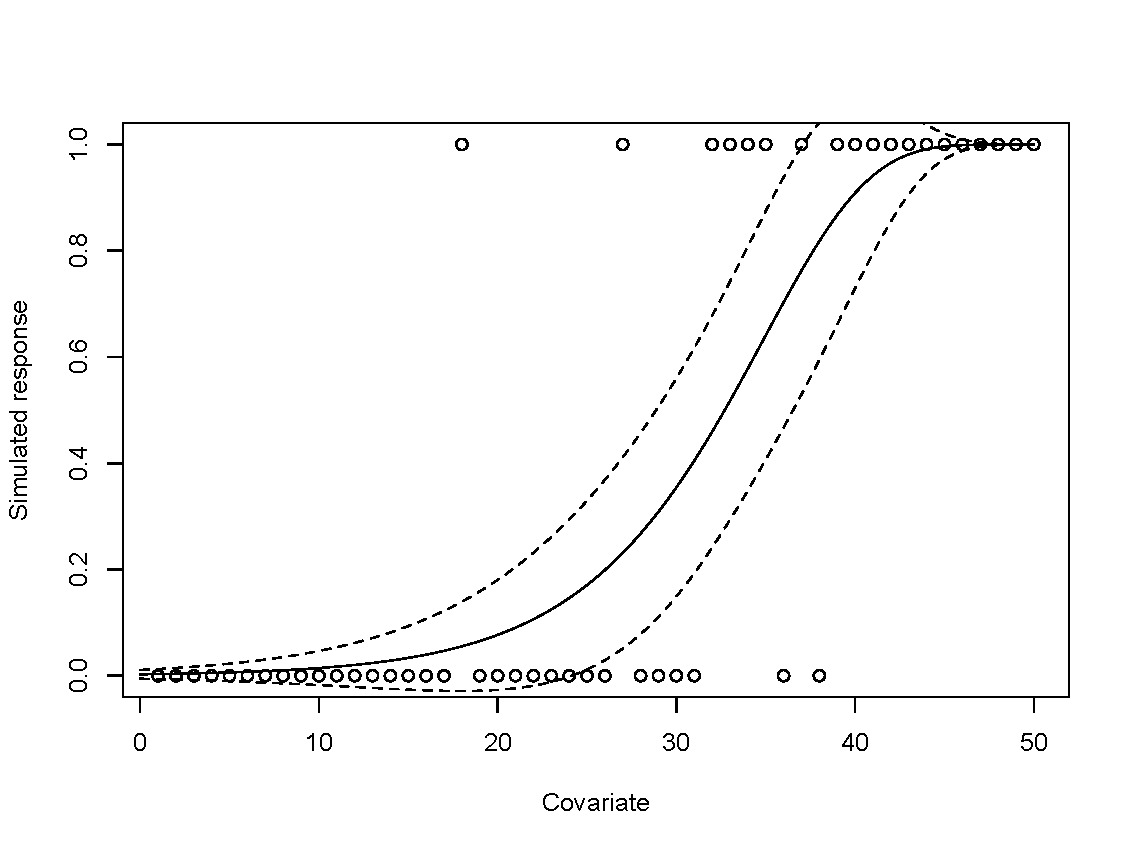
\includegraphics[width=.8\textwidth]{./figures/hw03_2_confidence.pdf}
      \label{fig:5}
    \end{figure}

\end{enumerate}


\end{document}
